% This is "sig-alternate.tex" V2.0 May 2012
% This file should be compiled with V2.5 of "sig-alternate.cls" May 2012
%
% This example file demonstrates the use of the 'sig-alternate.cls'
% V2.5 LaTeX2e document class file. It is for those submitting
% articles to ACM Conference Proceedings WHO DO NOT WISH TO
% STRICTLY ADHERE TO THE SIGS (PUBS-BOARD-ENDORSED) STYLE.
% The 'sig-alternate.cls' file will produce a similar-looking,
% albeit, 'tighter' paper resulting in, invariably, fewer pages.
%
% ----------------------------------------------------------------------------------------------------------------
% This .tex file (and associated .cls V2.5) produces:
%       1) The Permission Statement
%       2) The Conference (location) Info information
%       3) The Copyright Line with ACM data
%       4) NO page numbers
%
% as against the acm_proc_article-sp.cls file which
% DOES NOT produce 1) thru' 3) above.
%
% Using 'sig-alternate.cls' you have control, however, from within
% the source .tex file, over both the CopyrightYear
% (defaulted to 200X) and the ACM Copyright Data
% (defaulted to X-XXXXX-XX-X/XX/XX).
% e.g.
% \CopyrightYear{2007} will cause 2007 to appear in the copyright line.
% \crdata{0-12345-67-8/90/12} will cause 0-12345-67-8/90/12 to appear in the copyright line.
%
% ---------------------------------------------------------------------------------------------------------------
% This .tex source is an example which *does* use
% the .bib file (from which the .bbl file % is produced).
% REMEMBER HOWEVER: After having produced the .bbl file,
% and prior to final submission, you *NEED* to 'insert'
% your .bbl file into your source .tex file so as to provide
% ONE 'self-contained' source file.
%
% ================= IF YOU HAVE QUESTIONS =======================
% Questions regarding the SIGS styles, SIGS policies and
% procedures, Conferences etc. should be sent to
% Adrienne Griscti (griscti@acm.org)
%
% Technical questions _only_ to
% Gerald Murray (murray@hq.acm.org)
% ===============================================================
%
% For tracking purposes - this is V2.0 - May 2012

\documentclass{sig-alternate}

\begin{document}
%
% --- Author Metadata here ---
\conferenceinfo{CS 523 Multimedia Systems}{2017, University of Illinois at Chicago}
%\CopyrightYear{2007} % Allows default copyright year (20XX) to be over-ridden - IF NEED BE.
%\crdata{0-12345-67-8/90/01}  % Allows default copyright data (0-89791-88-6/97/05) to be over-ridden - IF NEED BE.
% --- End of Author Metadata ---

\title{Outpainting using Context Encoders and GAN}

%
% You need the command \numberofauthors to handle the 'placement
% and alignment' of the authors beneath the title.
%
% For aesthetic reasons, we recommend 'three authors at a time'
% i.e. three 'name/affiliation blocks' be placed beneath the title.
%
% NOTE: You are NOT restricted in how many 'rows' of
% "name/affiliations" may appear. We just ask that you restrict
% the number of 'columns' to three.
%
% Because of the available 'opening page real-estate'
% we ask you to refrain from putting more than six authors
% (two rows with three columns) beneath the article title.
% More than six makes the first-page appear very cluttered indeed.
%
% Use the \alignauthor commands to handle the names
% and affiliations for an 'aesthetic maximum' of six authors.
% Add names, affiliations, addresses for
% the seventh etc. author(s) as the argument for the
% \additionalauthors command.
% These 'additional authors' will be output/set for you
% without further effort on your part as the last section in
% the body of your article BEFORE References or any Appendices.

\numberofauthors{2} %  in this sample file, there are a *total*
% of EIGHT authors. SIX appear on the 'first-page' (for formatting
% reasons) and the remaining two appear in the \additionalauthors section.
%
\author{
% You can go ahead and credit any number of authors here,
% e.g. one 'row of three' or two rows (consisting of one row of three
% and a second row of one, two or three).
%
% The command \alignauthor (no curly braces needed) should
% precede each author name, affiliation/snail-mail address and
% e-mail address. Additionally, tag each line of
% affiliation/address with \affaddr, and tag the
% e-mail address with \email.
%
% 1st. author
\alignauthor
Shiwangi Singh\\
       \affaddr{Electronic Visualization Laboratory}
       \affaddr{University of Illinois at Chicago}\\
       \email{ssingh79@uic.edu}
% 2nd. author
\alignauthor
Shi Yin\\
       \affaddr{Electronic Visualization Laboratory}\\
       \affaddr{University of Illinois at Chicago}\\
       \email{syin8@uic.edu}
}
% There's nothing stopping you putting the seventh, eighth, etc.
% author on the opening page (as the 'third row') but we ask,
% for aesthetic reasons that you place these 'additional authors'
% in the \additional authors block, viz.
%\additionalauthors{Additional authors: John Smith (The Th{\o}rv{\"a}ld Group,
%email: {\texttt{jsmith@affiliation.org}}) and Julius P.~Kumquat
%(The Kumquat Consortium, email: {\texttt{jpkumquat@consortium.net}}).}
%\date{30 July 1999}
% Just remember to make sure that the TOTAL number of authors
% is the number that will appear on the first page PLUS the
% number that will appear in the \additionalauthors section.

\maketitle
\begin{abstract}
Image Extrapolation is necessary when parts of the image is missing and requires filling those missing gaps, we call this process as Outpainting. Semantics of a painting can be captured by neighbourhood pixel values which are basically contexts in an image. We build a model similar to semantic Inpainting except that we expand the image instead of filling in the missing gaps. We developed an extension of semantic Inpainting where we can retrieve image content around the borders and thus expand the image. Additionally, we built an interactive web interface where users can upload an image and test the model's capability to expand an image.
\end{abstract}

% A category with the (minimum) three required fields
\category{I.4.9}{Image Processing and Computer Vision}{Application}
%A category including the fourth, optional field follows...
\category{I.5.1}{Pattern Recognition}{Models}[Neural Nets]

\terms{Algorithms, Design, Theory}

\keywords{Deep Learning, Image Inpainting, Outpainting, Generative Adversarial Networks, Context Encoders}

\section{Introduction}
We have copious amount of historical images, black and white images and even digital images which have been deteriorated because of mishandling and corruption. Inpainting techniques are used to restore these deteriorated images by filling gaps. There are parametric and non-parameters methods in which one perform inpainting. Techniques that use \textit{Convolutional Neural Network} (CNN) are categorized as parametric approaches to inpainting. Due to the recent advances in the field of Image Generation~\cite{doersch2015unsupervised}, it only makes sense to use CNN and its variates to image inpainting.

Unsupervised deep learning has recently made it possible to answer questions pertaining image processing and image analysis such image denoising, image synthesis, image inpainting and so on. \textit{Generative Adversarial Networks} (GANs) were developed by Goodfellow et al. that allowed image generation in an unsupervised manner~\cite{goodfellow2014:generative}. Pathak et al. used the advantages of Context Encoders and GANs for semantic inpainting~\cite{pathak2016context}. Yeh et al. used contextual and perceptual loss in a Deep Convolutional GAN (DCGAN) like architecture for semantic inpainting further validating the importance of generative networks for inpainting~\cite{yeh2016:semantic}. This implementation was based on Pathak's work except that the use case is image expansion instead of hole filling inside the image.

\section{Context encoder and GAN}

\subsection{Architecture}

\subsubsection{Context Encoders}

There are two models used together for context inpainting. The first is the context encoder which is like a variation of denoising autoencoder for filling the missing region using the contextual information. Context encoder is an encoder-decoder model where encoder is used to learn high level representation of the data and the decoder is used to reconstruct the image from this abstract representation. As seen in Figure~\ref{fig:encoder} we have fully connected layers between encoders and decoders which takes a shape of 4000 units long vector. The input to the encoder is an image with missing borders and the output of the decoder is the filled borders. This output is regressed against the actual border cut outs. A binary mask is used for identifying the border regions which are dropped from the actual input to the model.

\begin{figure}[htb]
	\centering
	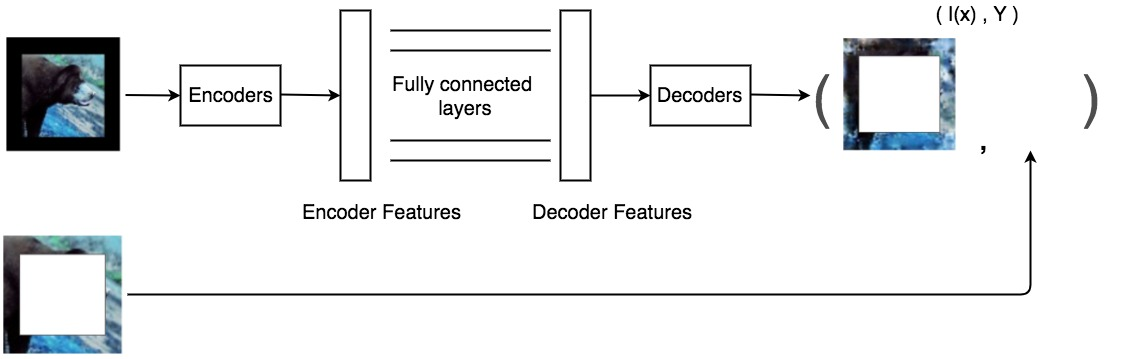
\includegraphics[width=0.5\textwidth]{encoder}
	\caption{Encoder-decoder model showing reconstruction loss}
	\label{fig:encoder}
\end{figure}

\begin{figure*}
	\centering
	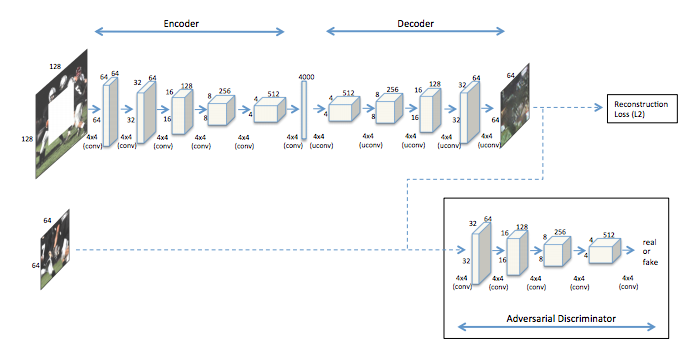
\includegraphics[width=16cm]{architecture}
	\caption{Model architecture as in~\cite{pathak2016context} except our inputs were as explained in Section~\ref{sec:imple}}
	\label{fig:archi}
\end{figure*}

\subsubsection{Generative Adversarial Networks (GANs)}

The output obtained from the context encoder model is not as sharp as we would like to achieve. To overcome the blurriness of the output and get a sharper result, we make use of GANs as seen in ~\cite{goodfellow2014:generative}. GANs consists of a Discriminator $D$ and a Generator $G$. The role of the Generator is to map a noisy distribution $Z$ to a data distribution $X$, this can be written as $G: Z \rightarrow X$. The role of the discriminator is to distinguish between the actual ground truth data and the predicted data by $G$. They basically play a game where $D$ tries to correct the model output and $G$ tries to confuse $D$ by showing the `fake' data as `real'. The following equation shows this mini-max game between $G$ and $D$:
\begin{equation}
	\min_{G}\max_{D}\mathbb{E}_{x\in\mathcal{X}}[\log(D(x))]+\mathbb{E}_{z\in\mathcal{Z}}[\log(1-D(G(z)))].
\end{equation}

For modeling the GANs, we use Generator as the Context Encoder model, and a adversarial Discriminator to identify between the real (ground truth) and the fake (decoder output) data. This can be seen in the bottom model in Figure~\ref{fig:archi}.

The architecture is adapted from AlexNet architecture~\cite{krizhevsky2012imagenet} with five convolutional layers with stride equal to two and five corresponding deconvolutional layers of hidden sizes (64, 32, 16, 8, 4). The filters used are of size 4*4. Figure~\ref{fig:encoder} shows the encoder and decoder shapes for the context encoder. The second type of model used for outpainting is GAN, where the input for the Discriminator comes from the context encoder model which is the predicted output borders and the ground truth borders, see Figure~\ref{??}. Again, the shape of the adversarial network consists of four convolutional layers taking a hidden shape of (32, 16, 8, 4) with 4*4 filters convolving the image.

\subsection{Loss Functions}
They use two kinds of losses used in the context encoder plus GANs model. The first is the reconstruction loss $\lambda_{rec}$ which is the L2 loss obtained from the Context encoder while regressing the context encoder model output to the actual missing borders. These losses are applied separately to the inputs and the missing regions. Thus a binary mask is used in the loss functions. The second kind of loss is the adversarial loss which is obtained from the discriminator. L2 tends to average together multiple modes in prediction whereas adversarial picks the mode from the distribution making the prediction look more real. Loss equations can be given as follows:
\begin{equation}
	L_{rec}(x) = ||M(x-F(1-M)x))||,
\end{equation}
\begin{equation}
	L_{adv} = \max_{D}\mathbb{E}_{x\in\mathcal{X}}[\log(D(x))+\log(1-D(F((1-M)x)))],
\end{equation}
and
\begin{equation}
	L = \lambda_{rec}L_{rec}+\lambda_{adv}L_{adv},
\end{equation}
where $L_{rec}$ is the total reconstruction loss, $L_{adv}$ is the adversarial loss and $L$ is the final joint loss.

\begin{figure}[htb]
	\centering
	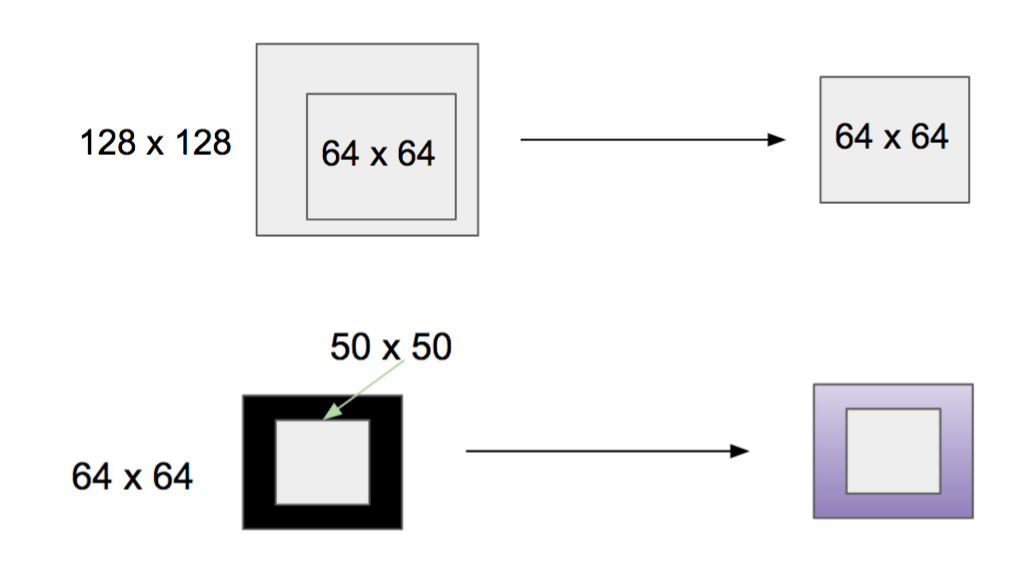
\includegraphics[width=9cm]{crop}
	\caption{Image cropping: (a) the random 64*64 selection from the resized image; (b) the missing borders (black) and the filled borders (purple)}
	\label{fig:crop}
\end{figure}

\begin{figure*}[htb]
	\centering
	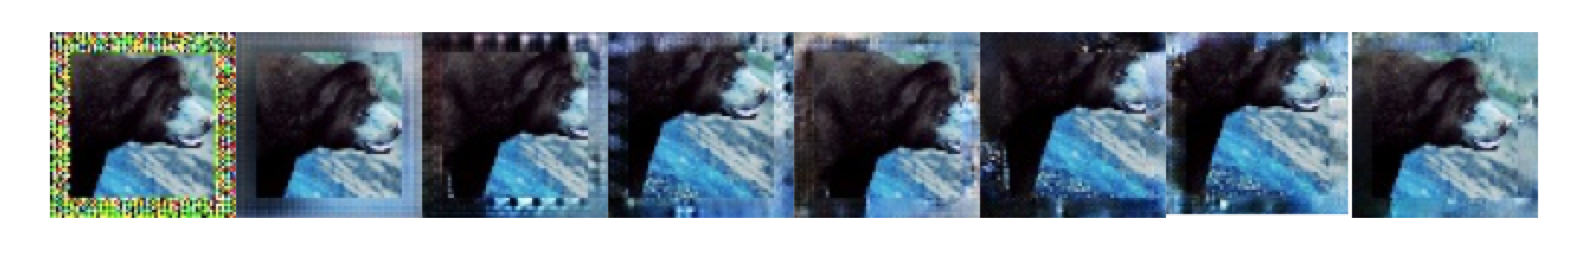
\includegraphics[width=16cm]{timestamp}
	\caption{Results obtained at various timestamps during the training process}
	\label{fig:time}
\end{figure*}

\section{Implementation}
\label{sec:imple}
Our system, written in Python and TensorFlow, consists of the following four modules: Image Loader module, Image Cropping module, GAN module, and UI module.

\subsection{Image Loader}
Our system firstly takes a set of images as input, and feeds it to \textit{Image Loader} module.

Image Loader module crops the maximum square region from the center of each input image. In other words, it ensures 1) the width (and height) of the cropped image is either the width or height of the original image, whichever is smaller, and 2) the center of the cropped image is also the center of the original image.

The cropped image then is scaled to 146*146. It randomly selects an 128*128 region from this 146*146 image. The RGB values are then mapped from $(0, 1)$ to $(-1, 1)$ linearly.

The set of these 128*128 images, noted as $TrainImage_{ori}$, is the output of Image Loader module, and is fed to Image Cropper module.

\subsection{Image Cropper}
\textit{Image Cropper} module's main functionality is two-fold. First, it produces input image set ($TrainImage$) for the generator by randomly picking a 64*64 square region in each image, and leaving the central 50*50 square of the 64*64 region intact while assigning black ((117, 104, 123) is used in our case) to the rest. Note that there is a 7-pixel wide `border' area in the 64*64 square region that is also assigned black color. This process is illustrated in Figure~\ref{fig:crop}. Second, it also produces input image set ($TrainCrop$) for the discriminator. The input set is simply the 64*64 square region with original values.

\subsection{GAN module}
\textit{GAN} module is where our core generative adversarial network resides, where our Generator is nothing but the Context Encoder model. The generator has five convolutional layers, with a Leaky ReLU layer after each of them. There there are five deconvolutional layers, with a ReLU layer after each one. The Discriminator, on the other hand, has four convolutional layers, also with a Leaky ReLU layer after each.

The output of each one of the models is used for computing the generative and the adversarial loss. Original reconstruction loss is calculated using the L2 loss function. Then using binary masks, the losses are calculated separately for the overlapping and the borders regions which are then summed together to obtain total Reconstruction loss. The objective function used in the GANs are sigmoid cross entropy with logits both for generative and adversarial parts of the model. The final loss is the joint loss making use of reconstruction loss and adversarial loss at the same time. The lambda values used for the reconstruction loss and for the adversarial loss are 0.9 and 0.1, respectively. The update function used is the Adam Optimizer with a learning rate of 0.0003 and a weight decay rate of 0.00001. The model is trained for 2000 epochs for approximately 48 hours.


\subsection{User Interface}
All the above-mentioned modules are for back-end computation. UI module is for front-end user interaction. The purpose of having a user interface is to allow users to upload their own images and view the output so that they have an intuitive way to evaluate our model.

\begin{figure}[htb]
	\centering
	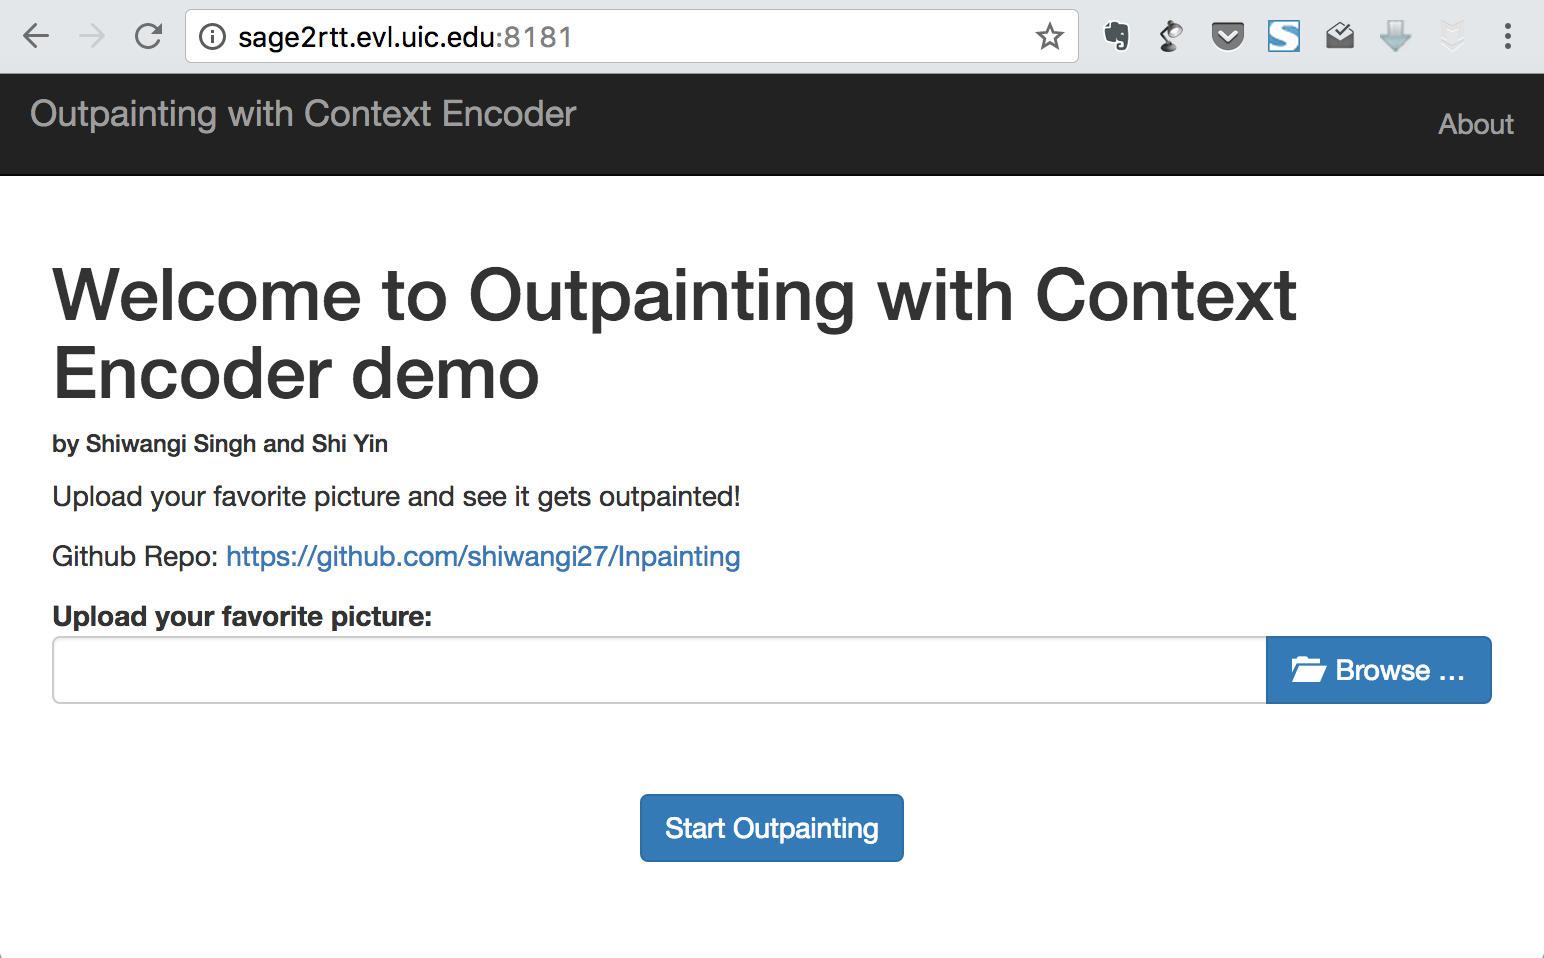
\includegraphics[width=8.5cm]{ui}
	\caption{User Interface of our system}
	\label{fig:ui}
\end{figure}

Figure~\ref{fig:ui} is an overview of our user interface. Users are allowed to upload any image file that has an extension of `png', `jpg' or `jpeg' from their local machine. Upon clicking on `Start Outpainting' button, the selected file will be uploaded to the system.

This image is fed into \textit{Image Loader} module and then \textit{Image Cropper} module to be processed, before GAN module finally produces a generated border to the intact central region of the uploaded image.


\begin{figure}[htb]
	\centering
	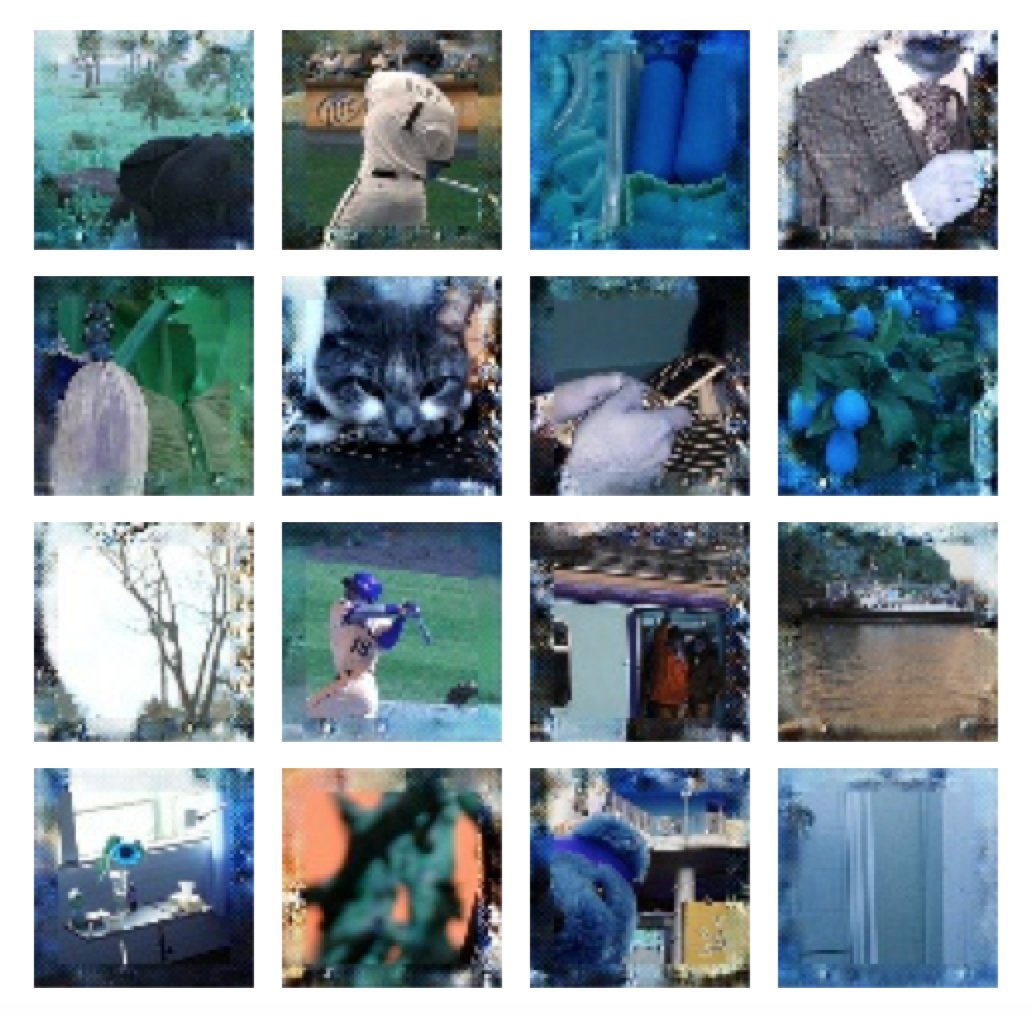
\includegraphics[width=8.5cm]{outResults}
	\caption{Results on test set after 2000 epochs}
	\label{fig:res}
\end{figure}

\section{Results}

We tested our GAN model on a data set that consists of 82,783 images retrieved from ImageNet database. We used 90\% of the downloaded images as training set, while the rest 10\% was used as test set.

We trained the data set for over 2000 epochs, with a learning rate of 0.0003 and a decay rate of 0.00001. Figure~\ref{fig:time} shows the results obtained at various timestamps during the training process.

Figure~\ref{fig:res} shows the results obtained on the test set. The borders painted are 7*7 in height and width in the 64*64 image. These borders were originally hidden or passed as black pixel values of 64*64 and the image content inside was 50*50.

Figure~\ref{fig:random} shows the model input and output of 8 randomly chosen images. The size of the input image is 50*50 (left) and the size of the output image is 64*64 (right). This result is obtained from a saved training model trained for 370 epochs.

\begin{figure}[htb]
	\centering
	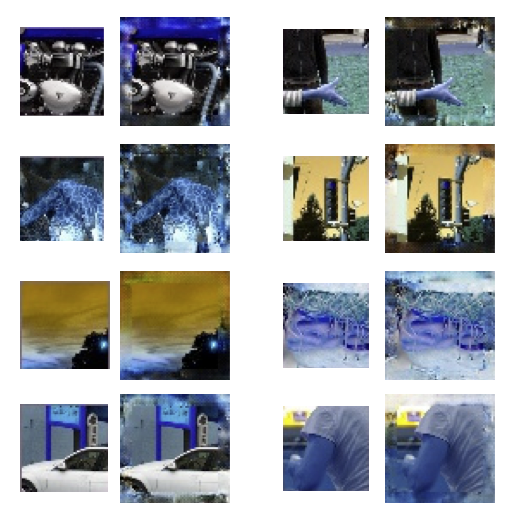
\includegraphics[width=8.5cm]{testResults}
	\caption{Comparison of model inputs and outputs}
	\label{fig:random}
\end{figure}

\section{Conclusion}
We used a context encoder model as a replacement for Generative network. This work required us to know a-priori about the ground truth which makes this model somewhat supervised. We needed an approach that was completely unsupervised for extrapolating images to a desired extent, shape and size, instead we were only able to outpaint image of fixed borders. In the future, we would like to use a GAN which is modeled to extrapolate the images and predict the neighborhood pixels using contextual information. Although, the results in that case wouldn't be as sharp as the one obtained by using context encoders. Sophisticated loss functions and trained models could be used to obtain competitive results for image outpainting. Furthermore, the interface allows us to interactively explore the capabilities of the model to generate outpainted images. This interface can be further extended to obtain outpainting of specified border shapes and sizes.

%\end{document}  % This is where a 'short' article might terminate

%
% The following two commands are all you need in the
% initial runs of your .tex file to
% produce the bibliography for the citations in your paper.
\bibliographystyle{abbrv}
\bibliography{sigproc}  % sigproc.bib is the name of the Bibliography in this case
% You must have a proper ".bib" file
%  and remember to run:
% latex bibtex latex latex
% to resolve all references
%
% ACM needs 'a single self-contained file'!
%

\end{document}
